\documentclass{article}
\usepackage[utf8]{inputenc}
\usepackage{array}
\usepackage{wrapfig}
\usepackage{multirow}
\usepackage{graphicx}
\usepackage{tabularx}
\usepackage{geometry}
\usepackage{changepage}


\makeatletter
%same as \subsubsection but @level 4
\renewcommand\paragraph{\@startsection{paragraph}{4}{\z@}%
{-3.25ex\@plus -lex \@minus -.2ex}%
{1.5ex \@plus .2ex}%
{\normalfont\normalsize\bfseries}}

% number \paragraph
\setcounter{secnumdepth}{4}

\makeatother


\title{\normalsize \texts{SOEN 6481 Summer 2021}\\ [1.0cm]
\large \textbf{\uppercase{Vision Document}}\\
\large \textbf{\uppercase{E-Concordia Drive}}
\normalsize \vspace*{2\baselineskip}\\
\textbf{Disclaimer:}
\textit{"I certify that this submission is the original and meets the Faculty's Expectations of Originality"}
}
%Title and Front page


\author{{Tavtej Singh Lehri}\\
{StudentID - 40121745}}

\begin{document}

\maketitle

\tableofcontents
\clearpage


\section{Introduction}
The purpose of this vision document is to collect and analyze all assorted ideas that have come up to define the system, its requirements with respect to consumers. Also, we shall predict and sort out how we hope this product will be used in order to gain a better understanding of the project, outline concepts that may be developed later, and document ideas that are being considered, but may be discarded as the product develops.\normalsize\vspace*{1\baselineskip}\\
In short, the purpose of this SRS document is to provide a detailed overview of our software product, its parameters and goals. This document describes the project's target audience and its user interface, hardware and software requirements. It defines how our client, team and audience see the product and its functionality. Nonetheless, it helps any designer and developer to assist in software delivery life-cycle (SDLC) processes.\normalsize\vspace*{1\baselineskip}\\
E-Concordia drive is an E-learning platform for students to learn and practice driving lessons to obtain a license. It has got three main users: Trainer, Student and Admin.
Admin edits, comments, approves and publishes  lessons uploaded by a trainer.
Once approved the content is ready to be viewed by students.

\subsection{References}
[1] Improvement of Detection for Warning Students in E-learning Using Web Cameras - Scientific Figure on ResearchGate. Available from: https://www.researchgate.net/figure/A-block-diagram-of-the-e-learning-system\_fig1\_275541493 [accessed 13 Jul, 2021]


\section{Positions}

\subsection{Problem Statement}

\begin{table}[h!]
\begin{tabular}{|p{4.5cm}|p{11.5cm}|}
\hline
\textbf{The Problem of} & Not being able to hold in-person learning and practice for obtaining driver's license due to COVID-19 \\ \hline
\textbf{Affects} & All people who are new to driving and existing course students. \\ \hline
\textbf{The impact of which is} & That due to the pandemic the driving school had to close the in-person classes. \\ \hline
\textbf{The Solution to which is} & Creating an E-Learning website using which, the students can watch training videos prepared by instructors. Also based on the training module students can solve quizzes, which will help them practice for the main exam.\\ \hline
\end{tabular}
\caption{Problem Statement}
\label{table:1}
\end{table}

\subsection{Product Position Statement}


\begin{tabular}{|p{4.5cm}|p{11.5cm}|}
\hline
\textbf{For} & All people who are new to driving and existing course students\\ \hline
\textbf{Who}& Want to practice for the final driving exam.\\ \hline
\textbf{The E-Concordia Drive} & is an e-learning web product\\ \hline
\textbf{That} & helps students prepare for their final writing test, while sitting at their home.\\ \hline
\textbf{Unlike} & attending school amidst of the pandemic \\ \hline
\textbf{Our Product} & Helps the student learn from the vicinity of their homes. Using this platform they have access to videos 24/7, which helps revisit the videos them with if they did not understand something at first. Apart from this the platform also helps with practice quizzes.\\ \hline
\end{tabular}

\section{Stakeholder Description}

\subsection{Stakeholder Summary}


\begin{tabular}{|p{4.5cm}|p{4.5cm}|p{6.5cm}|}
\hline
\textbf{Name} & \textbf{Description} & \textbf{Responsibilities} \\ \hline
Business Analyst & Is a person responsible for the SRS document and understanding the business needs & Should prepare SRS document and any changes to it, understand the business requirements, understand the customer requirements, layout clear and precise requirements for the developers and testers.\\ \hline
Architects & Acts as development lead and is a guy who has knowledge of MVC architecture  & Create the MVC style architecture for the developers, communicate with business and clients to design and execute solutions. Make executive software design decisions\\ \hline
Developers & Coders of the website & They are responsible to write a stable, understandable and easily executable PHP language based website. Should be familiar with MVC architecture. Should be able to read and understand requirements from the requirement document\\ \hline
Database Admins & Is a person who maintains and develops database for the application. & Should be familiar with MySQL database. Responsible for creating and maintaining the database. Should have in-depth knowledge of SQL.\\ \hline
QA/Test Analyst & Is a person who can find bugs in the application and help achieve stable application & Should be familiar with JIRA, can create test suite, test plan, test cases.\\ \hline
Marketing \& Advertising & A firm responsible to bring the application to end user. & Select the target users, advertise to the users, maintain social media advertising and help in SEO. \\ \hline
\end{tabular}


\subsection{User Summary}

\begin{tabular}{|p{3.5cm}|p{3.5cm}|p{4.5cm}|p{4cm}|}
\hline
\textbf{Name} & \textbf{Description} & \textbf{Responsibilities} & \textbf{Stakeholder}\\ \hline
Students &  & & \\ \hline
Teachers &  & & \\ \hline
Admin &  & & \\ \hline
Students &  & & \\ \hline
Students &  & & \\ \hline

\end{tabular}

\subsection{User Environment}
\begin{itemize}
    \item\textbf{Tools used for the project:}
    \begin{itemize}
        \item \textbf{PhpStorm:} IDE for software development
        \item \textbf{JIRA:} To improve the management of new development and defects.
        \item \textbf{GitHub:} for configuration management of the source code, test code and data.
        \item \textbf{MySQL:} for creating and maintaining the data.
        \item \textbf{Overleaf:} for creating all project related documentations
    \end{itemize}
    \item\textbf{Team Structure:}
    \begin{itemize}
        \item There will be 1 software architect who will also act as the development manager. The development team will consist of 4-5 developers and will be lead by the architect. Number of developers will go down to 2 once the project is live.
        \item The testing team will have 4 testers. The 4 people includes a test lead and 3 test analysts. Number of testers will reduce to 1-2 once the project goes live.
        \item There will be 1 scrum master and 1 business analyst.
        \item 1 developer and 1 tester will be moved to maintenance team once the project is live and deal wil production issues. 
    \end{itemize}
    \item Development of the product will be done using agile methodologies. It will be divided in 3 iterations. Iteration 1 will be 8 weeks long, Iterations 2 and 3 each will be 4 weeks long.
    \item For this release the project will work on Google Chrome and Safari. Expansion of this project will see working on other web browsers available in the market. Also there is a plan to create an application after analyzing the response for the website.
    \item Users should have a browser enabled device for using the website. Also the devices they use should be capable of viewing video and audio clips.
    \item Marketers and Advertisers should be familiar with the SEO and SCO tools. They should track all the social media activities via twitter, facebook and instagram.
    \item Student users shall have access to all the videos and quizzes once they enroll for the course.
    \item Trainer users should be able to record, manage and publish the videos for the approval of admin. Also they should be able to create quizzes for students to practice.
    \item Admin shall have the access to approve/reject the published stuff by the trainers.
\end{itemize}

\subsection{Key Stakeholder or Users Needs}


\begin{tabular}{|p{2.5cm}|p{2.5cm}|p{3.5cm}|p{3.5cm}|p{3.5cm}|}
\hline
\textbf{Need} & \textbf{Priority} & \textbf{Concerns} & \textbf{Current Solution} & \textbf{Proposed Solution}\\ \hline

Login Page & High &  & None & Create a sign-up page where users can create profiles as per their roles.\\ \hline
Receive notification when new video is uploaded & High & Volume of notifications & & \\ \hline
Responsive Website & Medium & Website should respond to user's behavior and environment. & None & Use of HTML and CSS style coding for the front end. \\ \hline
Stable and Bug Free website & High & There will be defect leakage & None & Use the extensive testing technique, track the defects in JIRA, perform regression testing after each iteration. \\ \hline


\end{tabular}


\section{Product Overview}

\subsection{Product Perspectives}
Below is the block diagram for the e-learning website:
\begin{figure}[htb!]
    \centering
    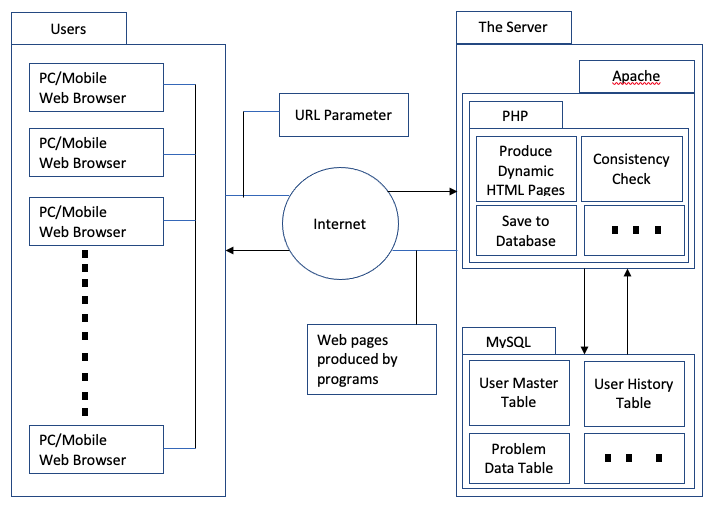
\includegraphics[scale=0.4]{1.png}
    \caption{A block diagram of the e-learning system [1] }
    \label{fig:my_label}
\end{figure}


\subsection{Assumptions and Dependencies}

\begin{tabular}{|p{5.5cm}|p{6.5cm}|}
\hline
\textbf{Assumptions} & \textbf{Dependencies} \\ \hline
Who & What\\ \hline

\end{tabular}

\section{Product Features}
\textbf{Below listed are all the high level features of the website:}
\begin{enumerate}
    \item \textbf{Sign-Up:} All the end users should be able to create an account.
    \item \textbf{Login:} After the sign-up is complete, students will be given a studentID and traffic No, using this they can login. Teachers and Admins can login with the username and password provided by the institute.\\[0.5ex]
    
    \textbf{Students:}
    \item \textbf{Dashboard:}The dashboard page should have the general information about the type of license a student is training for.
    \item There will be 3 status of the modules: Completed,In Progress and Pending. Students cannot bypass the lessons and have to go sequentially.
    \item \textbf{Start Again} feature allows the student to preview the lesson contents again. Note: it will be available only after the lesson is complete.
    \item Lesson icons will have the slides count and the duration from the lesson content. This will help students track their individual lesson progress as well.
    \item Left pane will have the Student ID and Examination ID along with next exam date, expiry dates of lesson and fees.
    \item Lessons will have an interactive screen. This will enable touchscreen device users no navigate easily. Videos will adjust to screen orientation of the mobile device.
    \item Description box will contain any extra information that the students nee to know.
    \item Volume adjustment button will be provided for the users to keep volume as per their need.
    \item Start button starts the video slides. Once the start button is clicked two new buttons will appear which will help students navigate through slides
    \item Students when they logout will resume from where they left and will not have to start over again.
    \item Quiz related to the lesson will be enabled once a student completes their training video.
    \item Correct answer will be highlighted in green when students select the answer. If the student answer a wrong answer the answer will be marked in red and correct answer will be displayed in green.
    \item For match the following and rearranging the correct sequence, drag and drop feature will be provided.\\[0.5ex]
    
    \textbf{Trainers and Admins:}
    \item Dashboard page for the teacher login will have navigation pane with following links: Home, All Lessons, Pending, Drafts, Published, Notification. Navigation pane will be on all the pages in teacher account.
    \item Quick navigation will show the categorized number of all lessons, drafts, pending, notifications
    \item All lessons link will take the users to all lessons page where the trainer will have manage lessons button.
    \item Manage lessons button will open a popover form where teacher will input the Lesson name(drop down menu as per SRS from EDC server), description, language (language listing as per SRS from EDC server) and icon to upload(using choose file button).
    \item Submit button in the popover form enables trainer to insert the content to lesson.
    \item A new pane is created in all lessons page for the lesson created with 5 buttons namely, Slide, Quiz,Lesson Status, Edit and Delete.
    \item Slide button is used for slide creation, Quiz button for quiz creation, lesson status shows the status of lesson in creation(Draft, Pending and Published). Edit and Delete.
    \item Plus button is used to expand the lesson and see the contents of it and lesson information pane on the right.
    \item when clicked on slide button the website will open an slide editor popover form.
    \item Media type in slide form will be audio, video and image. Slide duration is auto detected.
    \item Media file can be selected using the choose file button. Slide description is suitable for LTR or RTL.
    \item Slides are added after the user clicks on submit. The entry will have an icon for the notification on changes done by admin.
    \item Addition of Quiz also opens a popover pane. Quiz type will enable to select the type of quiz from, true/false, Right Answer, Drag and Drop and Reorder.
    \item For True/False space will be provided for trainer to type the question and provide the correct answer using dropdown.
    \item For choose correct answer Area to type question is given or it can be based on media(A/V or Image). 4 Answers will be typed in and the correct answer radio button will be selected by trainer.
    \item For drag and drop Questions will be typed in and matching answer will be given. System will shuffle the answers once the student is attempting the quiz.
    \item When trainer click on draft link on the navigation pane system navigates to the draft lessons page, where all the drafts are listed.
    \item When trainer click on published link on the navigation pane system navigates to the published lessons page, where all the published are listed.
    \item When the trainer click on notification, they will be navigated to the notifications page. It will display all the updates done either by trainer or admin.
    \item There will be 3 status of the updates: lesson updated(lesson creation, pending, draft and published), comment updated(when trainer updates admin comments), quality comment(from admin for trained)
    \item View button against the comments will take trainer to the slides having admin comments on it. Status of comment will change to done once changes are made and admin will be notified.
    \item Trainers will be allowed to create versions of the lessons they created using the edit button in the lesson management.
    \item If one trainer is busy creating a lesson, the trainer who is free will be given a lesson editing access and it will be displayed which trainer is working on which lesson.
    \item Once the lesson is published trainer will loose access to edit or delete the slide and admin will have control over it.
    \item Admin has access to accept/reject students. Once a trainer leaves the school, admin can remove them from the system.
    
\end{enumerate}

\section{Other Product Requirements}

\end{document}
